\documentclass[c]{beamer}

%\usepackage[frenchb]{babel}
%\usepackage[T1]{fontenc}
\usepackage[utf8]{inputenc}
%\usepackage{graphicx}

\title[Intermediary defense of Industrial Project]{Implementation of the OpenHart workflow in DAE platform}
\author{Julien BIDOLET, Clément AUDAM and Pierre P\'EZOT }
\date{7 septembre 2013}
\institute{TELECOM Nancy}
\titlegraphic{
\includegraphics[width=2.5cm]{telecom_nancy.png}
\hspace{1cm}

\includegraphics[width=2.5cm]{loria.jpg}
}


\usetheme{Warsaw}
%\usecolortheme{spruce}

\addtobeamertemplate{footline}{\insertframenumber/\inserttotalframenumber}

\begin{document}


\begin{frame}
  \maketitle
\end{frame}

\begin{frame}
  \tableofcontents
\end{frame}

%\section{Introduction}

%\begin{frame}
%  \begin{block}{Introduction}
    %\begin{itemize}
%	During the third year of Telecom Nancy, students have to realize an industrial project. We choose to apply to a project about creating a reusable environment for research benchmarking in automated handwriting recognition.
    %\end{itemize}
%  \end{block}
%  \begin{figure}
%    
\includegraphics[width=4cm]{loria}
%  \end{figure}
%\end{frame}

\section{Context}
\subsection{OpenHart}
\begin{frame}
	\frametitle{OpenHart}
	\begin{block}{OpenHart}
	\begin{itemize}
		\item OpenHart is competitive exam set up by the National Institute of Standards and Technology.
		\item Teams of developers are evaluated on their performance in handwriting documents transcription and translation.
		\item The evaluation tool is not really handy.
	\end{itemize}
	\end{block}
\end{frame}
\subsection{QGAR}
\begin{frame}
   \frametitle{ QGAR }
   \begin{block}{QGAR}
   \begin{itemize}
	   \item QGAR is a research team of the laboratory “Loria”.
	   \item They are working in the area of graphics recognition and document analysis.
	   \item Implementation the OpenHart evaluation system on DAE platform.   
	\end{itemize}
	\end{block}
\end{frame}

\subsection{What we had to do}

\begin{frame}
   \frametitle{ What we had to do}
   \begin{block}{People inveloved}
	\begin{itemize}
	   \item Bart LAMIROY (QGAR)
	   \item Jean-François SCHEID (Télécom Nancy)
	   \item Clément AUDAM, Julien BIDOLET, Pierre PEZOT
	 \end{itemize}
	\end{block}
	\begin{block}{Proof of concept}
	Proof of concept: OpenHart implementation on the DAE platform using web services.
	\\Organization:
	   \begin{itemize}
		   \item Meetings
		   \item Working time
		   \item Tools
	   \end{itemize}
	\end{block}
	\end{frame}
			    

\section{Project Progress}

\subsection{DAE Analysis}
\begin{frame}

\frametitle{Our work}
\framesubtitle{DAE Analysis}
\begin{block}{The goal}
Create and link two simple web-services : 
\begin{itemize}
\item Generate a list of random images URL in DAE
\item For each, download and rotate the image
\end{itemize}
\end{block}
\begin{block}{Attempts to communicate with DAE}
\begin{itemize}
\item Use pre-generated URL to send a request
\item Use the WSDL representation of web-services
\item Simply execute web-services with Taverna
\end{itemize}
\end{block}
\end{frame}
\subsection{OpenHart Analysis}
\begin{frame}
\frametitle{Our Work}
\framesubtitle{OpenHart Analysis}
\begin{block}{The goal}
Modeling the OpenHart evaluation process with Taverna
\end{block}
\begin{block}{Tasks}
\begin{itemize}
\item Create a simple model of OpenHart's pipeline
\item Web services specifications
\item Understand and document metrics for the algorithms' evaluation
\item Try to understand the algorithm of a participant
\end{itemize}
\end{block}
\end{frame}
\subsection{Problems encountered}
\begin{frame}
\frametitle{Our work}
\framesubtitle{Problems encoutenred}
\begin{block}{DAE communication protocols}
\begin{itemize}
\item Difficult to use different tools
\item Insufficient communication
\end{itemize}
\end{block}
\begin{block}{Difficult to understand how the OpenHart pipeline works}
\begin{itemize}
\item Few documentation
\item Complicated makefile
\end{itemize}
\end{block}
\end{frame}
\section{Upcoming work}
\subsection{Planned work}
\begin{frame}
\frametitle{Upcoming work}
\framesubtitle{Planned Work}
The timetable has changed
  \begin{figure}
  \begin{center}
    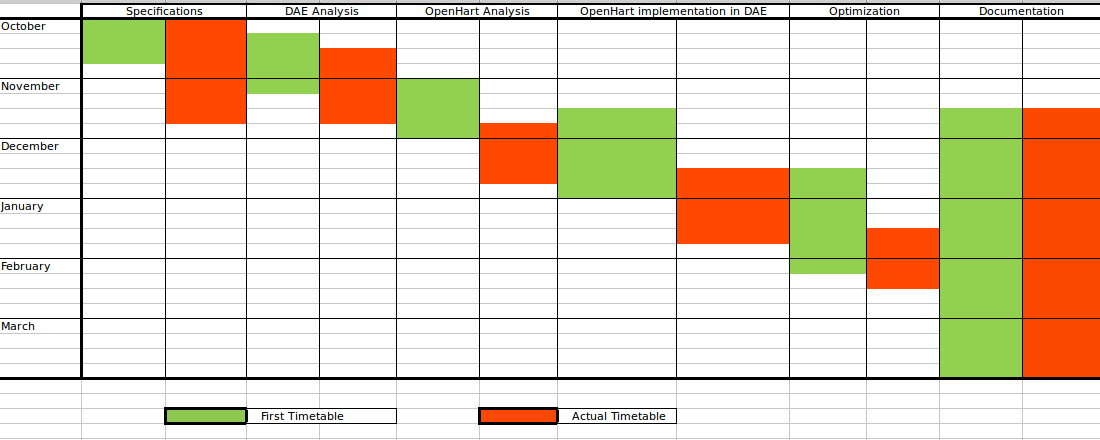
\includegraphics[width=10cm]{planning.png}
	\newline
	Timetable comparison
  \end{center}
  \end{figure}
\end{frame}

\subsection{What we are going to do}

\begin{frame}
\frametitle{Upcoming work}
\framesubtitle{What we are going to do}
\begin{block}{Implement OpenHart in DAE}
\begin{itemize}
	\item Implement algorithms running
	\item Implement metrics
\end{itemize}
\end{block}

\begin{block}{Optimization}
	\begin{itemize}
	\item Write an optimizations manual
	\item Optimize!
	\end{itemize}
\end{block}

\begin{block}{Documentation}
Keep documenting the code
\end{block}
\end{frame}

\section{Conclusion}
\begin{frame}
  \begin{block}{Conclusion}
    %\begin{itemize}
   Even if we haven’t finished the project, we have already learned a lot about project management and organization.

   We would like to thanks Bart Lamiroy and Jean-François Scheid for their help.
	%\end{itemize}
  \end{block}
  \begin{figure}
    
\includegraphics[width=4cm]{loria}
  \end{figure}
\end{frame}
\end{document}
